\documentclass[12pt]{article}

\usepackage{sbc-template}
\usepackage{graphicx,url}
\usepackage[utf8]{inputenc}
\usepackage[brazil]{babel}
\usepackage{float}
\usepackage{placeins}

\sloppy

\title{Redes Orientadas a Conteúdo: Fundamentos, Arquiteturas e Aplicações Práticas}

\author{Rodolfo A. Silva\inst{1}, João Victor J. Assis\inst{2}, Alex de O. Alves\inst{3}}


\address{Instituto de Matemática e Computação - Universidade Federal de Itajubá (UNIFEI)}

\begin{document} 

\maketitle

\begin{abstract}
The current Internet model, based on end-to-end communication and IP addresses, faces increasing scalability and efficiency challenges due to high data consumption. This work presents Content-Oriented Networks (CONs) as a viable alternative to this model, focusing on information identification rather than its physical location. Through a literature review and analysis of architectures such as NDN and CCN, the pillars of CONs are discussed: hierarchical naming, name routing, native caching, and data-centric security. The study also addresses practical applications in IoT and streaming, as well as analyzing the challenges of implementation and scalability. It concludes that, although requiring profound structural changes, CONs offer a robust foundation for the future generation of networks.
\end{abstract}
     
\begin{resumo} 
  O atual modelo da Internet, baseado na comunicação fim-a-fim e em endereços IP, enfrenta desafios crescentes de escalabilidade e eficiência diante do grande consumo de dados. Este trabalho apresenta as Redes Orientadas a Conteúdo (ROC) como uma alternativa viável a esse modelo, focando na identificação da informação e não na sua localização física. Por meio de uma revisão bibliográfica e análise de arquiteturas como NDN e CCN, discutem-se os pilares das ROCs: nomeação hierárquica, roteamento por nomes, cache nativo e segurança centrada no dado. O estudo aborda ainda aplicações práticas em IoT e streaming, além de analisar os desafios de implementação e escalabilidade. Conclui-se que, embora exijam mudanças estruturais profundas, as ROCs oferecem uma base robusta para a futura geração de redes.
\end{resumo}


\section{Introdução}

As Redes Orientadas a Conteúdo mudam significativamente as regras de roteamento, onde agora o foco é o nome do centeúdo e não mais o endereço do hospedeiro ou da máquina \cite{jacobson2009networking}. Tais regras de roteamento permitem criar um arquitetura mais eficiente para a distribuição de conteúdo, resultando em um compartilhamento eficiente de conteúdo e de dados, aumento na disponibilidade do conteúdo e também, suporte à segurança do conteúdo.

\subsection{Problemas do Modelo Atual}

A arquitetura atual da Internet já foi desenvolvida a alguns anos com o objetivo de conectar computadores para o compartilhamento de recursos e comunicações entre as estações. Esse modelo é baseado no paradigma fim-a-fim, onde a regra é onde a informação está. 
Como hoje o uso da rede mudou drasticamente, sendo a internet usada principalmente para a disseminação e recuperação de conteúdos nomeados, como vídeos e arquivos em nuvens, o modelo centrado em localização enfrenta dificuldades para lidar com essa nova realidade.

Tais gargalos estão ligados à escabilidade e gerenciamento, onde o modelo enfrenta dificuldades em gerenciar um grande volume de dados e usuários, e também a mobilidade e segurança, uma vez que o modelo ligado a localização amarra o conteúdo à sua localização física, complicando a mobilidade do conteúdo e a sua segurança, dependendo da segurança do canal e não do dado em si \cite{ambiel2013redes}.

\subsection{Introdução às Redes Orientadas a Conteúdo (ROC)}

Como alternativa para superar tais gargalos citados no ponto anterior, surge um novo paradigma chamado Redes Orientadas a Conteúdo, que sugere o conteúdo sendo tratado como elemento primitivo da rede, independente da sua localização física \cite{ambiel2013redes}.

Nas ROCs a infraestrutura da rede participa de forma ativa no armazenamento e na distribuição. O usuário solicita um conteúdo pelo nome e a rede é responsável por encontrar a cópia mais próxima, aumentando a eficiência da entrega e a disponibilidade da informação \cite{brito2012redes}.

Essa evolução não é apenas uma melhoria incremental, mas uma tentativa de reconstruir a arquitetura da rede para que ela seja compatível com a forma que a socidade consome a informação hoje: de forma massiva.

\section{Referêncial Teórico}

\subsection{Histórico e a Crise do Modelo Host-to-Host}

A arquitetura TCP/IP foi consolidada em uma era onde a comunicação era predominante entre dois pontos fixos. O objetivo principal era a força da conexão entre as estações e não a eficiência da distribuição em massa \cite{clark1988design}.

Uma vez que a internet se popularizou, o tráfego de informações se tornou assimétrico e focado em conteúdo. A internet atual tenta resolver problemas de disseminação de conteúdo através de camadas de aplicação, gerando uma complexidade desnecessária do uso dos recursos de rede, uma vez que a camada de rede permanece "cega" ao que transporta \cite{ahlgren2012survey}. Além disso, no modelo atual, o mesmo dado atravessa o núcleo de rede várias vezes para atender usuários diferentes. A mobilidade é um entrave. Como o endereço IP define tanto a identidade, quanto a localização, quando um dispositivo troca de rede, sua identidade lógica muda, interrompendo o fluxo de dados.

\subsection{Arquiteturas de Referências: CCN e NDN}

O marco inicial das ROCs foi o projeto Contect Centric Networking (CCN) \cite{jacobson2009networking}. Esse projeto evoluiu para Named Data Networking (NDN), umas das arquiteturas mais estudadas atualmente.

A arquitetura NDN baseia-se em dois pacotes fundamentais: Interest Package, onde o consumidor coloca o nome do conteúdo desejado em um pacote de "interesse" e espalha pela rede e o Data Package, onde o nó que possui o conteúdo responde com o pacote de "Dados", que é autenticado por uma assinatura criptográfica.

\section{Conceitos Fundamentais das Redes Orientadas a Conteúdo}

\subsection{O que são Redes Orientadas a Conteúdo}

As Redes Orientadas a Conteúdo (ROCs) ou \textit{Content-Oriented Networks} (CON), representa um novo paradigma de comunicação para a Internet. Diferente da arquitetura tradicional baseada no protocolo IP, onde o foco está na comunicação entre hospedeiros, identificados por endereços. As ROCs concentram-se diretamente no conteúdo solicitado na requisição.

Nas ROCs, não é necessário conhecer a localização física ou lógica do conteúdo solicitado, mas apenas seu identificador. Assim, a rede é responsável por localizar, recuperar e entregar o conteúdo pedido, independentemente de onde ele esteja armazenado. 

Essa mudança representa uma evolução na forma padrão de uso da Internet, que passou de um modelo centralizado na comunicação entre máquinas para um modelo onde o foco é o consumo de informação, como vídeos, imagens e serviços digitais.

\FloatBarrier
\subsection{Principais Conceitos}

As Redes Orientadas a Conteúdo introduzem uma série de conceitos fundamentais importantes para garantir um bom funcionamento dessa nova arquitetura. Dentre os principais, destacam-se:

\begin{itemize}
\item \textbf{Nomeação de Conteúdo:}
Nas ROCs, cada conteúdo é identificado por um nome único, ao invés de um endereço IP. Esses nomes podem ser estruturados de forma hierárquica, semelhante a URLs, permitindo melhor organização e agregação de dados, facilitando a persistência do conteúdo.

\item \textbf{Roteamento Baseado em Nomes:}
As ROCs utilizam os nomes dos conteúdos como base para o roteamento, isso permite que o conteúdo seja obtido de múltiplas fontes, como caches intermediários ou servidores distribuídos.

\item \textbf{Armazenamento em Rede (In-Network Caching):}
Esse conceito permite que os nós da rede armazenem conteúdos que trafegam por eles, possibilitando que futuras requisições pelo mesmo conteúdo sejam respondidas mais rapidamente por esse nós, aumentando a eficiência e a disponibilidade dos dados \cite{bvm12}. Isso melhora algumas limitações da Internet atual, como problemas de escalabilidade, mobilidade e eficiência na distribuição de conteúdo.

\item \textbf{Segurança Baseada no Conteúdo:}
Diferentemente do modelo tradicional, onde a segurança está associada à conexão, nas ROCs a segurança é aplicada ao conteúdo, garantindo integridade e autenticidade dos dados independentemente da fonte que realizou a resposta.

\end{itemize}
\begin{table}[htbp]
\centering
\caption{Comparação entre a arquitetura tradicional da Internet e o modelo de Redes Orientadas a Conteúdo.}
\label{tab:comparacao}
\begin{tabular}{|l|l|l|}
\hline
\textbf{Aspecto} & \textbf{Internet Tradicional} & \textbf{ROC} \\ \hline
Identificação & Endereço IP & Nome do conteúdo \\ \hline
Modelo & Cliente-servidor & Centrado em conteúdo \\ \hline
Roteamento & Baseado em localização & Baseado em nome \\ \hline
Cache & Limitado (CDN) & Nativo na rede \\ \hline
Segurança & Baseada na conexão & Baseada no conteúdo \\ \hline
\end{tabular}
\end{table}

\section{Arquiteturas de Redes Orientadas a Conteúdo}

As Redes Orientadas a Conteúdo não possuem uma única forma de implementação. Ao longo dos anos, diferentes propostas de arquitetura foram desenvolvidas com o objetivo de viabilizar esse novo paradigma de comunicação, cada uma com suas particularidades, mas todas baseadas no conceito central de acesso ao conteúdo por meio de nomes, e não de endereços \cite{bvm12}.

Em geral, essas arquiteturas buscam resolver problemas como escalabilidade, eficiência na distribuição de dados e suporte à mobilidade, propondo mudanças na forma como o conteúdo é identificado, roteado e armazenado na rede \cite{ambiel2013redes}.

\subsection{Principais Arquiteturas}

Dentre as diversas propostas existentes, algumas se destacam por sua relevância na literatura e por servirem como base para pesquisas na área:

\begin{itemize}

\item \textbf{CCN / NDN (Content-Centric Networking / Named Data Networking):}
Essa é uma das abordagens mais conhecidas e estudadas. Nela, a comunicação ocorre por meio de dois tipos principais de pacotes: \textit{Interest} (requisição) e \textit{Data} (resposta). O usuário solicita um conteúdo pelo nome, e a rede é responsável por encontrar e retornar esse dado, podendo obtê-lo de caches intermediários \cite{jacobson2009networking}.

\item \textbf{DONA (Data-Oriented Network Architecture):}
Essa arquitetura propõe um sistema baseado em identificadores persistentes para conteúdos, utilizando uma estrutura de resolução para localizar os dados na rede. O foco principal está na persistência e na segurança da informação \cite{bvm12}.

\item \textbf{NetInf (Network of Information):}
O NetInf trabalha com a ideia de objetos de informação independentes de localização, utilizando mecanismos de resolução de nomes para encontrar o conteúdo desejado. Essa abordagem também considera aspectos de mobilidade e distribuição eficiente \cite{bvm12}.

\item \textbf{PSIRP (Publish-Subscribe Internet Routing Paradigm):}
Baseado no modelo de publicação e assinatura (\textit{publish/subscribe}), o PSIRP permite que usuários recebam conteúdos de interesse sem precisar conhecer sua origem. Esse modelo é eficiente para aplicações orientadas a eventos \cite{bvm12}.

\end{itemize}

Essas arquiteturas mostram diferentes formas de implementar o paradigma das ROCs, mas todas compartilham a ideia central de abstrair a localização dos dados e focar no conteúdo em si.


\subsection{Funcionamento Básico}

Apesar das diferenças entre as arquiteturas, o funcionamento geral das Redes Orientadas a Conteúdo segue um fluxo semelhante.

Primeiramente, o usuário realiza uma requisição informando o nome do conteúdo desejado. Essa requisição é encaminhada pela rede por meio dos roteadores, que utilizam estruturas internas para decidir qual o melhor caminho para localizar o conteúdo \cite{ambiel2013redes}.

Durante esse processo, a rede pode encontrar o conteúdo em diferentes pontos, como em caches intermediários ou no servidor de origem. Caso o conteúdo seja encontrado em um nó mais próximo do usuário, ele é retornado diretamente, reduzindo o tempo de resposta e o tráfego na rede.

\begin{figure}[htbp]
\centering
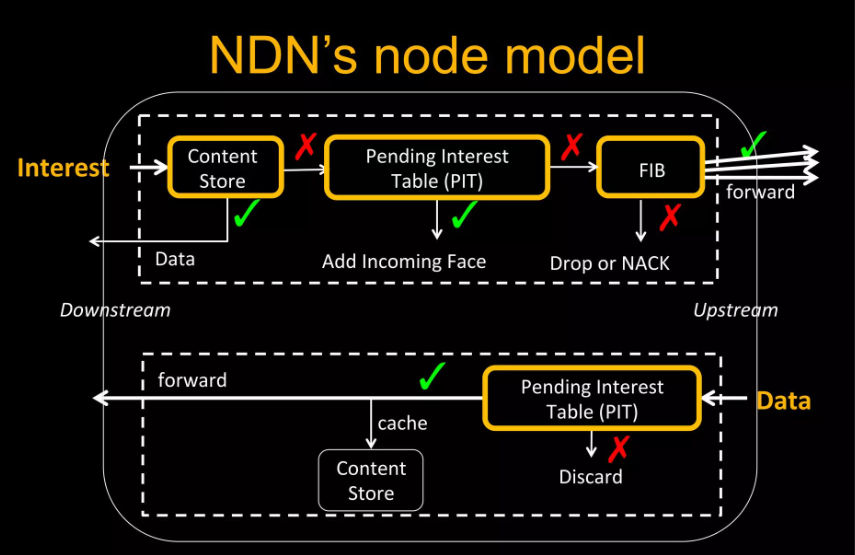
\includegraphics[width=0.8\linewidth]{figuras/ndn_model.png}
\caption{Fluxo básico de funcionamento das Redes Orientadas a Conteúdo, mostrando o envio de requisições por nome e o retorno do conteúdo a partir da fonte mais próxima.}
\label{fig:funcionamento-roc}
\end{figure}

Observa-se que o conteúdo pode ser retornado por diferentes caminhos, dependendo da localização das cópias disponíveis na rede. Esse comportamento é um dos principais fatores que contribuem para a eficiência das ROCs.

\subsection{Componentes Principais}

Para que esse modelo funcione, os roteadores das ROCs possuem estruturas adicionais em comparação aos roteadores tradicionais. No caso da arquitetura CCN/NDN, destacam-se três componentes principais:

\begin{itemize}

\item \textbf{Content Store (CS):}
Responsável por armazenar conteúdos em cache dentro do roteador, permitindo que requisições futuras sejam atendidas diretamente.

\item \textbf{Pending Interest Table (PIT):}
Armazena as requisições pendentes de conteúdo, permitindo que o roteador saiba para onde enviar a resposta quando o dado for encontrado.

\item \textbf{Forwarding Information Base (FIB):}
Utilizada para encaminhar as requisições com base no nome do conteúdo, funcionando de forma semelhante às tabelas de roteamento da Internet tradicional, porém baseada em nomes.

\end{itemize}

Esses componentes permitem que os roteadores atuem de forma mais inteligente, participando ativamente do processo de distribuição de conteúdo, o que representa uma das principais diferenças em relação ao modelo tradicional de redes \cite{ambiel2013redes}.

\section{Tipos de Serviços em Redes Orientadas a Conteúdo}

A flexibilidade arquitetural das ROCs, aliada às funcionalidades nativas de roteamento por nomes, segurança baseada no conteúdo e armazenamento em rede, viabiliza uma ampla gama de serviços que dificilmente poderiam ser implementados com a mesma eficiência no modelo tradicional da Internet. Nesta seção, são apresentados os principais tipos de aplicações que se beneficiam desse paradigma, organizados em quatro grandes grupos: distribuição de conteúdo, sistemas distribuídos, IoT e redes móveis, e aplicações baseadas em eventos.

\subsection{Distribuição de Conteúdo}

A distribuição massiva de conteúdo é, provavelmente, o domínio no qual as ROCs apresentam seus benefícios mais imediatos. Como o modelo opera essencialmente sobre o ato de localizar e entregar dados nomeados, a entrega de mídia passa a ser tratada como uma funcionalidade nativa da rede, eliminando camadas complexas de intermediação presentes na arquitetura atual.

\begin{itemize}

\item \textbf{Streaming}
O \textit{streaming} de conteúdo em tempo real, como transmissões esportivas, \textit{lives} de redes sociais e aulas síncronas, envolve a entrega simultânea de um mesmo fluxo para um grande número de usuários. Em redes IP tradicionais, essa demanda é tratada por soluções como CDNs e \textit{multicast}, que, embora funcionais, exigem infraestrutura complementar. Nas ROCs, o armazenamento em rede e a agregação de requisições similares na \textit{Pending Interest Table} (PIT) possibilitam que um único fluxo seja replicado eficientemente entre os roteadores, reduzindo drasticamente a carga no servidor de origem \cite{ahlgren2012survey}.

\item \textbf{Vídeo sob Demanda:}
Serviços de \textit{streaming} e compartilhamento de vídeos apresentam um padrão de consumo em que uma pequena parcela do catálogo concentra a maior parte das requisições, comportamento frequentemente descrito por distribuições de Zipf. Esse cenário é especialmente favorecido pelo cache em rede das ROCs: ao identificar conteúdos populares, os roteadores passam a manter cópias locais, reduzindo a latência percebida pelo usuário e o tráfego entre redes \cite{bvm12}. Adicionalmente, a nomeação hierárquica permite estratégias sofisticadas de \textit{prefetching} e de atualização incremental de segmentos de mídia.

\end{itemize}

\subsection{Sistemas Distribuídos}

Aplicações distribuídas modernas exigem mecanismos eficientes para localizar dados espalhados em múltiplos pontos de processamento e armazenamento. As ROCs fornecem, de maneira nativa, uma infraestrutura que desacopla o conteúdo de sua localização física, característica especialmente útil em arquiteturas distribuídas contemporâneas.

\begin{itemize}

\item \textbf{Cloud Computing:}
Em ambientes de computação em nuvem, os dados podem estar replicados em diferentes \textit{datacenters} distribuídos geograficamente. Nas redes IP, a recuperação desses dados depende de balanceadores de carga, DNS geográfico e políticas de roteamento baseadas em endereços. Já nas ROCs, o simples ato de solicitar um conteúdo pelo nome permite que a rede localize a réplica mais próxima, reduzindo latência e melhorando a tolerância a falhas sem exigir intervenção das camadas superiores \cite{ambiel2013redes}.

\item \textbf{Edge Computing:}
A computação de borda aproxima o processamento dos usuários, visando reduzir a latência e aliviar o núcleo da rede. As ROCs são particularmente alinhadas a esse paradigma, uma vez que seus roteadores, ao atuarem como nós de cache e de encaminhamento inteligente, podem implementar naturalmente funcionalidades de borda. Conteúdos frequentemente requisitados passam a ser disponibilizados em pontos próximos ao consumidor, e fluxos críticos podem ser direcionados a instâncias regionais de processamento apenas pelo uso adequado da nomeação hierárquica.

\end{itemize}

\subsection{IoT e Redes Móveis}

A proliferação de dispositivos conectados e a crescente demanda por conectividade móvel expõem limitações estruturais do modelo baseado em endereços IP. As ROCs oferecem respostas arquiteturais a esses desafios.

\begin{itemize}

\item \textbf{Mobilidade Facilitada:}
No modelo IP, o endereço de um dispositivo atua simultaneamente como identificador e como localizador, o que faz com que qualquer mudança de rede resulte em ruptura das conexões ativas ou na necessidade de protocolos auxiliares, como o \textit{Mobile IP}. Nas ROCs, a identificação é atribuída ao conteúdo, e não ao dispositivo. Dessa forma, um usuário que migre entre redes Wi-Fi e celular, por exemplo, continua a receber os dados solicitados sem necessidade de reestabelecer conexões ou lidar com mecanismos específicos de mobilidade \cite{ahlgren2012survey}.

\item \textbf{Dispositivos Conectados (IoT):}
A Internet das Coisas envolve bilhões de sensores e atuadores, muitos deles com recursos computacionais e energéticos limitados. O modelo tradicional exige que cada dispositivo possua um endereço único e se baseie em protocolos adicionais para configuração, descoberta e segurança. Nas ROCs, dispositivos podem simplesmente publicar ou consumir dados nomeados, aproveitando a segurança nativa baseada em assinaturas criptográficas e o cache em rede para reduzir o consumo energético. Esses fatores são especialmente relevantes em cenários como cidades inteligentes, monitoramento ambiental e sistemas industriais \cite{bvm12}.

\end{itemize}

\subsection{Aplicações Baseadas em Eventos}

Aplicações modernas frequentemente operam sobre modelos reativos, nos quais o envio e o consumo de informações dependem de eventos específicos, e não de uma comunicação contínua entre pares. As ROCs mostram-se particularmente adequadas a esses cenários.

\begin{itemize}

\item \textbf{Publish/Subscribe:}
O paradigma \textit{publish/subscribe} constitui a base de arquiteturas como a PSIRP, na qual os consumidores manifestam interesse por tópicos ou classes de conteúdo, e a rede se encarrega de encaminhar novas publicações aos assinantes adequados. Esse modelo elimina a necessidade de que o produtor conheça explicitamente seus consumidores, o que é vantajoso em sistemas distribuídos, notificações em tempo real e aplicações de mensageria em larga escala \cite{bvm12}.

\item \textbf{Conteúdo Multimídia e Aplicações Modernas:}
O trabalho de \cite{bvm12} destaca que as ROCs também se mostram promissoras para aplicações contemporâneas que combinam conteúdo multimídia, interatividade e distribuição em massa, como jogos em nuvem, ambientes de realidade virtual colaborativa e plataformas sociais de larga escala. Nesses cenários, a combinação entre nomeação expressiva, cache distribuído e mecanismos nativos de segurança fornece subsídios para reduzir latência, aumentar a escalabilidade e simplificar a implementação quando comparada ao modelo IP.

\end{itemize}

\section{Estudo de Caso: NDN Testbed Global}

Para ilustrar a aplicabilidade prática das Redes Orientadas a Conteúdo em um ambiente real, adota-se como estudo de caso o \textit{Named Data Networking Testbed}, iniciativa consorciada que reúne diversas universidades de pesquisa internacionalmente reconhecidas, sob liderança da \textit{University of California, Los Angeles} (UCLA). Esse \textit{testbed} constitui um dos exemplos mais maduros de implantação prática de uma arquitetura de ROC em escala intercontinental \cite{afanasyev2018brief}.

\subsection{Contexto e Motivação}

O projeto NDN teve origem em 2010 como uma das propostas financiadas pela \textit{National Science Foundation} (NSF), no âmbito do programa \textit{Future Internet Architecture} (FIA), que buscava repensar os fundamentos da Internet em resposta às limitações do modelo IP \cite{zhang2014ndn}. O consórcio reuniu pesquisadores de instituições como UCLA, \textit{University of Arizona}, \textit{Colorado State University}, \textit{Washington University in St. Louis}, \textit{University of Memphis}, \textit{University of Illinois at Urbana-Champaign}, \textit{Michigan State University}, \textit{Tsinghua University} e \textit{Beijing Institute of Technology}, entre outras.

A motivação central do projeto consistia em validar, em condições realistas, se os princípios teóricos das ROCs — nomeação de conteúdo, roteamento por nomes, cache em rede e segurança por assinatura — seriam capazes de sustentar aplicações contemporâneas em larga escala, e não apenas em simulações controladas.

\subsection{Arquitetura e Implementação}

O NDN Testbed é composto por nós distribuídos em diferentes países da América do Norte, Europa e Ásia. Cada nó atua como um roteador NDN, implementando as três estruturas fundamentais da arquitetura: a \textit{Content Store} (CS), a \textit{Pending Interest Table} (PIT) e a \textit{Forwarding Information Base} (FIB). A comunicação entre os nós utiliza túneis sobre o protocolo IP, o que permite a convivência com a infraestrutura atual da Internet sem exigir modificações nos roteadores intermediários.

O software de referência adotado é o NFD (\textit{Named Data Networking Forwarding Daemon}), desenvolvido pelos próprios membros do consórcio e mantido como projeto de código aberto. A segurança do conteúdo é implementada por meio de assinaturas digitais vinculadas à nomenclatura hierárquica, permitindo que qualquer nó ou usuário valide a autenticidade dos dados sem depender da fonte original \cite{afanasyev2018brief}.

\subsection{Aplicações Avaliadas}

Sobre esse ambiente foram desenvolvidas e avaliadas diversas aplicações representativas, dentre as quais destacam-se:

\begin{itemize}

\item \textbf{NDN-RTC:}
Sistema de videoconferência em tempo real desenvolvido para funcionar diretamente sobre a arquitetura NDN, explorando o cache em rede para reduzir o consumo de banda em cenários com múltiplos participantes.

\item \textbf{ndnSIM:}
Simulador integrado ao NS-3, amplamente utilizado pela comunidade acadêmica para avaliar novos algoritmos de roteamento, estratégias de encaminhamento e políticas de cache em redes NDN.

\item \textbf{NDN-IoT:}
Conjunto de experimentos voltados à integração da arquitetura com dispositivos de Internet das Coisas, avaliando o desempenho em redes de sensores e em aplicações de monitoramento ambiental.

\end{itemize}

\subsection{Resultados e Lições Aprendidas}

Os experimentos conduzidos ao longo dos anos demonstraram que, em cenários de distribuição de conteúdo popular, o cache em rede proporcionou redução significativa na latência percebida pelos usuários e no consumo de banda entre os nós, corroborando as expectativas teóricas sobre as ROCs \cite{zhang2014ndn}. Em aplicações envolvendo mobilidade, observou-se que os consumidores puderam migrar entre diferentes pontos de acesso sem perda perceptível no fluxo de dados, uma vez que as requisições subsequentes são simplesmente reemitidas sob o mesmo nome de conteúdo.

Por outro lado, os experimentos também expuseram desafios não triviais. A escalabilidade da FIB em cenários com um número elevado de prefixos nomeados exigiu o desenvolvimento de estruturas de dados mais sofisticadas, como árvores de prefixos otimizadas e filtros probabilísticos \cite{afanasyev2018brief}. Questões relacionadas à padronização da nomeação entre domínios administrativos distintos, bem como à coexistência com o IP durante uma eventual migração gradual, permanecem como temas de pesquisa em aberto.

\subsection{Relevância para o Estudo das ROCs}

O NDN Testbed consolida-se como referência prática para o estudo das ROCs por reunir, em um mesmo ambiente, os principais componentes discutidos ao longo deste trabalho: nomeação hierárquica, roteamento baseado em nomes, cache em rede e segurança centrada no conteúdo. Além disso, a adesão de universidades de pesquisa reconhecidas internacionalmente confere robustez metodológica ao conjunto de resultados produzidos, reforçando o argumento de que as ROCs representam uma alternativa viável e cientificamente fundamentada às limitações do modelo atual da Internet.

\section{Aplicação no Mundo Real}

Devido à não utilização do potencial computacional oferecido pelos avanços nas tecnologias dos dispositivos na rede, como os roteadores modernos, o modelo atual da internet, que se concentra na interação entre servidores de conteúdo e usuários, encontrará obstáculos com a crescente quantidade de conteúdo acessível.

Uma forma possível é o uso de Content Centric Network (CCN), combinada com Scalable Video Coding (SVC), técnica que codifica vídeos em camadas de modo que separa uma camada básica (BL) e camadas avançadas (EL).

A popularidade do conteúdo é levada em consideração para determinar se ele é armazenado no cache da estação de base. Quando a popularidade alcança um certo nível, a estação base faz o cache e informa suas estações vizinhas sobre esse conteúdo. As estações vizinhas armazenam a informação recebida em uma tabela conhecida como NCS (Neighbors Content Store). Essa tabela contém os dados necessários para encaminhar a solicitação à estação base que possui o conteúdo armazenado fisicamente \cite{gta_icn_2019}.

\begin{figure}[H]
    \centering
    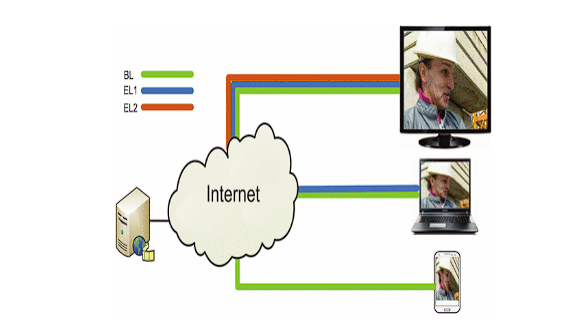
\includegraphics[width=0.5\linewidth]{figuras/caseReal.png}
    \caption{Transmissão de vídeo codificado em SVC para dispositivos diversos. Fonte: \cite{gta_icn_2019}.}
    \label{fig:placeholder}
\end{figure}

\section{Desafios e Limitações}

Apesar das vantagens apresentadas anteriormente das Redes Orientadas a Conteúdo, esse paradigma ainda enfrenta desafios significativos, como: escalabilidade, nomeção, consistência dos dados, infraestrutução da rede atua e eficiência para o roteamento.
\begin{itemize}

\item \textbf{Escalabilidade:}
Um dos principais desafios está relacionado à escalabilidade. O número de conteúdos disponíveis na rede é muito maior do que o número de dispositivos, o que torna difícil o gerenciamento e o roteamento baseado em nomes.

\item \textbf{Nomeação de conteúdos:}
Outro ponto crítico é a nomeação de conteúdos, que com a ausência de um padrão universal pode dificultar a identificação do mesmo conteudo entre diferentes sistemas e impactar o desempenho do roteamento.

\item \textbf{Consistência de cache:}
Sobre o uso dos caches, embora traga benefícios de desempenho, pode gerar problemas com a consistência e atualização dos conteúdos, especialmente em cenários onde os dados são frequentemente modificados.

\item \textbf{Mudanças na infraestrutura:}
Outro fator relevante é a necessidade de mudanças na infraestrutura atual da Internet. A inserção das ROCs exige alterações significativas na arquitetura de rede e nos protocolos existentes, o que dificulta sua implementação em larga escala e sua integração com os sistemas já estabelecidos.

\item \textbf{Eficiência do roteamento:}
Por fim, a eficiência do roteamento baseado em nomes ainda é uma incognita, já que o aumento da quantidade de conteúdos pode impactar o roteamento e o desempenho dos roteadores.
\end{itemize}

\section{Conclusões}

A análise realizada neste trabalho permite concluir que as Redes Orientadas a Conteúdo (ROCs) não representam apenas uma melhoria incremental, mas uma mudança essencial para a sustentabilidade da Internet. Enquanto o modelo tradicional baseado em endereços IP \cite{clark1988design} demonstra sinais de exaustão diante do grande tráfego de dados, as ROCs propõem uma arquitetura onde o conteúdo é o elemento principal, não ligado mais à sua localização física \cite{ambiel2013redes}.

Os benefícios identificados, como o armazenamento nativo em rede (\textit{in-network caching}) e o roteamento baseado em nomes, se mostram fundamentais para otimizar a distribuição de mídia e reduzir a latência em serviços críticos \cite{brito2012redes}. Além disso, a segurança centrada no dado, conforme proposto pela arquitetura NDN \cite{jacobson2009networking}, oferece uma resposta concreta às vulnerabilidades do modelo focado em canais de comunicação, garantindo a integridade da informação independentemente da fonte de entrega.

Contudo, a transição para esse novo modelo não é fácil. Conforme discutido, desafios relacionados à escalabilidade das tabelas de roteamento e à padronização da nomeação hierárquica ainda demandam pesquisas \cite{afanasyev2018brief}. A evolução da rede ocorrerá de forma gradual, possivelmente através de modelos híbridos que integrem as vantagens das ROCs às redes legadas.

Sendo assim, as Redes Orientadas a Conteúdo oferecem uma base sólida e eficiente para as demandas da sociedade da informação. O fortalecimento deste modelo é um passo estratégico para viabilizar o futuro de uma rede verdadeiramente escalável e segura.
\bibliographystyle{sbc}
\bibliography{sbc-template}

\end{document}
